\documentclass[conference]{IEEEtran}

\usepackage{listings}
\usepackage[framed,numbered,autolinebreaks,useliterate]

%\documentclass[draftcls, 12pt,onecolumn,oneside]{IEEEtran}
\usepackage{cite,graphicx,amssymb,amsmath,color,textcomp}
\newtheorem{theorem}{\underline{Theorem}}%[section]
\newtheorem{lemma}{\underline{Lemma}}%[section]
\newtheorem{remark}{\underline{Remark}}%[section]
\ifCLASSOPTIONcompsoc

\usepackage[nocompress]{cite}
\else
\usepackage{cite}
\fi
\newcounter{mytempeqncnt}

\begin{document}


\title{Design and Simulation of a Weak Signal Detection Algorithm: Multiple Signal Sending Algorithm}
\author{Zilong Wang 18281218\\wangzilong@bjtu.edu.cn
 }


\maketitle
\begin{abstract}
The communication between the earth and the moon is obscured by the noise. Since the noise that produced by the long-distance interference is inevitable, an algorithm for the weak signal detection, which is called the multiple signal sending algorithm, is designed for the purpose of solving this de-noise problem in the following content. The key of the multiple signal sending algorithm is to send and receive one signal for many times, and consequently the accuracy of received signals can be improved significantly. The results of simulation that shown below proved the validity of the multiple signal sending algorithm.
\end{abstract}

\begin{IEEEkeywords}
weak signal detection system, de-noise problem, earth-moon communication, simulation
\end{IEEEkeywords}


\section{Introduction}
The technology of weak signal detection is widely used in radar, communication, sonar, earthquake and industrial measurement\cite{b1}.

In free space, if a spherical wave is radiated at the transmitting point, the power at the receiving point would be $P_r=\frac{P_t}{d^2}$, where $P_r$ is the power at the receiving point, $P_r$ is the power at the transmitting point and $d$ is the distance between the two points. Considering the distance between the moon and the earth is $384,400$km, the power at the receiving point is extremely weak. Compared with noises, the amplitude of the useful signal is weak and completely obscured by the noise\cite{b2}.

At present, a weak signal detection algorithm is important in the communication between earth and moon. In this paper, we will focus on the multiple signal sending algorithm and its simulation.



\section{Related Work}
\subsection{ALE-FFT Algorithms\cite{b3}}
The FFT acquisition is a normal method in this case and ALE-FFT algorithm, which ALE is added before FFT, can enhance the ability of weak signal detection, especially for the weak signal which has big dynamic range of Doppler frequency. In residual carrier acquisition mode, the ALE is equivalent to an adaptive band-pass filter which enhances the acquisition signal noise ratio(SNR) greatly.

\subsection{Wavelet Transform\cite{b4}}
The basic meaning of Wavelet Transform(WT) is the x signal through the scale and shift, decomposing to a series of sub-frequency with the different spatial resolution, the different frequency characteristics and the directional characteristic innertube signal, this innertube signal has a good time domain, a frequency band and other partial characteristics. Therefore the wavelet analysis to signal has an excellent detection performance under low SNR.


\section{The Proposed Method}
\subsection{Problem Description}
Given the signal $x(n)$ sent from moon where $x(n)=\pm 1$ with equal probability. $\omega(n)$ is white gaussian noise and $\omega(n)$ obeys $N(0,1)$. Suppose $y(n)$ is the signal received on earth, we have:
\begin{equation*}
y(n) = hx(n) + \omega(n)
\end{equation*}
where $h$ is the weaken ratio of the signal traveling from moon to earth. In this problem, $h = 10^{-3}$. The problem is to recover $x(n)$ from $y(n)$.

\subsection{Multiple Signal Sending Algorithm}
The $\omega(n)$ is always an independent variable obeys $N(0,1)$. If we send each signal for $N$ times, The sum of $\omega(n)$ would be much smaller than the sum of $hx(n)$ for $N$ times due to Central Limit Theorem\cite{b5}. Taking $n=1$ as an example:

\begin{equation}
y(n) = h\,x(1)+\omega(n)
\end{equation}

We calculate the sum of $y(n)$ and \textbf{OP(1)} can be developed as follows \textbf{OP(2)}:
\begin{equation}
\sum^N_1 y(n) = Nhx(1)+\sum^N_1 \omega(n)
\end{equation}

When $N$ is large enough, we can recover x(n) from y(n) by the sign of $\sum^N_1y(n)$. If $\sum^N_1y(n) \ge 0$, we can interpret $x(n)$ from $y(n)$ as $1$. In contrast, if $\sum^N_1y(n) < 0$, we can interpret $x(n)$ from $y(n)$ as $-1$.


\section{Simulation}
In this section, we study the effect of Multiple Signal Sending Algorithm by analyzing the \emph{Bit Error Ratio} (BER) versus $N$ by the simulation.

We employ a signal array $\textbf{X}=[x_1,x_2,...,x_{10^3}]$ where $\textbf{x}_i=\pm 1$ with equal probability. A noise array $\textbf{W}=[\omega_1,\omega_2,...,\omega_{10^3}]$ is used, where $\omega_i$ is $N$ sum of single gaussian noise obeying $N(0,1)$. Then we can get the input signal array $\textbf{Y}=[y_1,y_2,...,y_{10^3}]$ by the following equation:
\begin{equation*}
\textbf{Y}=Nh\textbf{X}+\textbf{W}
\end{equation*}

If $y_i$ is positive, then we assume $y_i$ is $1$. Otherwise $y_i$ is $-1$. Comparing $x_i$ and $y_i$ respectively and calculating the BER. We simulate different $N$ and the figure of BER versus $N$ as follows Fig. \ref{fig}.
\begin{figure}[htbp]
\centering
\vspace{-4mm}
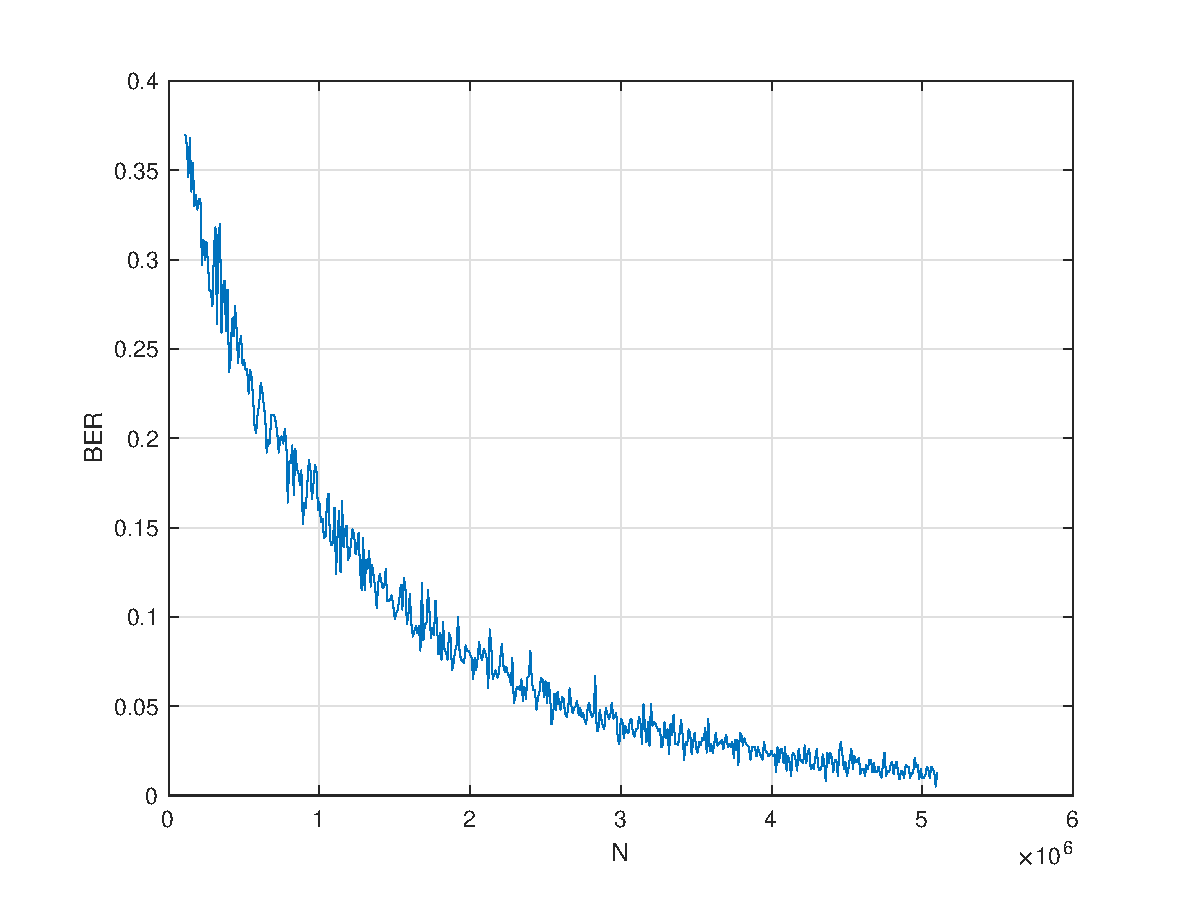
\includegraphics[height=48mm,width=64mm]{BERvsN.eps}
\vspace{-4mm}
\caption{BER vs. $N$}
\centering
\label{fig}
\vspace{-4mm}
\end{figure}

\subsection{Comparing of different $h$}
From \textbf{OP(2)} we find:
\begin{equation*}
\begin{cases}
Nhx \ \propto\  k_1N\\
\sum^N_1 \omega(n) \ \propto\  k_2\sqrt{N}\\
\end{cases}
\end{equation*}
where $k_1$ and $k_2$ are constant. So if $h$ is reduced by $10$ times, then $N$ should be expanded by $100$ times.

Here is the simulation with different $h$:


\begin{tabular}{cc}
\centering
\includegraphics[height=30mm,width=40mm]{1e-3.eps}&
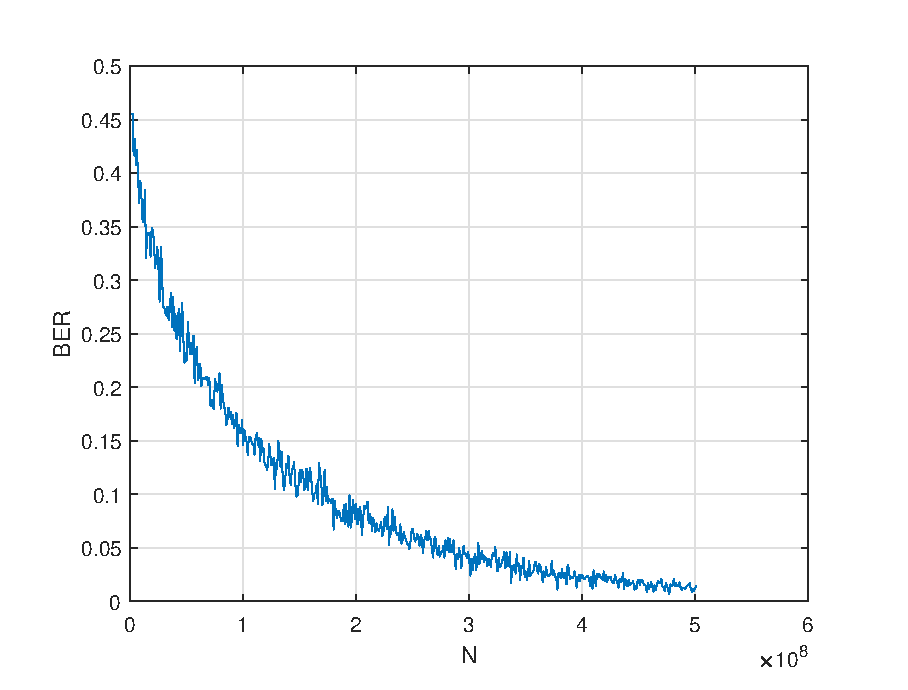
\includegraphics[height=30mm,width=40mm]{1e-4.eps}\\
$h=10^{-3}$ & $h=10^{-4}$\\
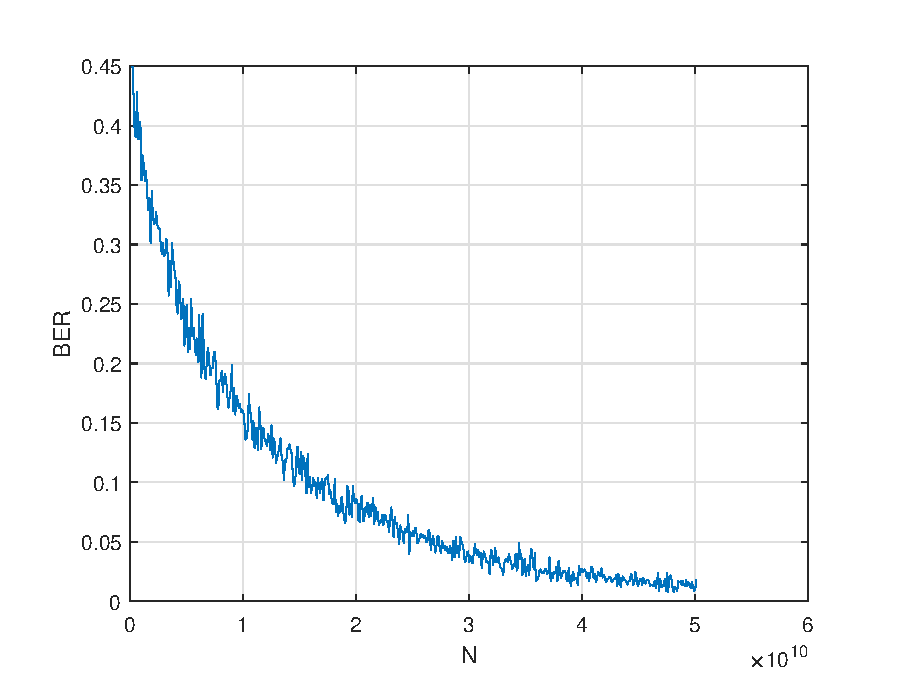
\includegraphics[height=30mm,width=40mm]{1e-5.eps}&
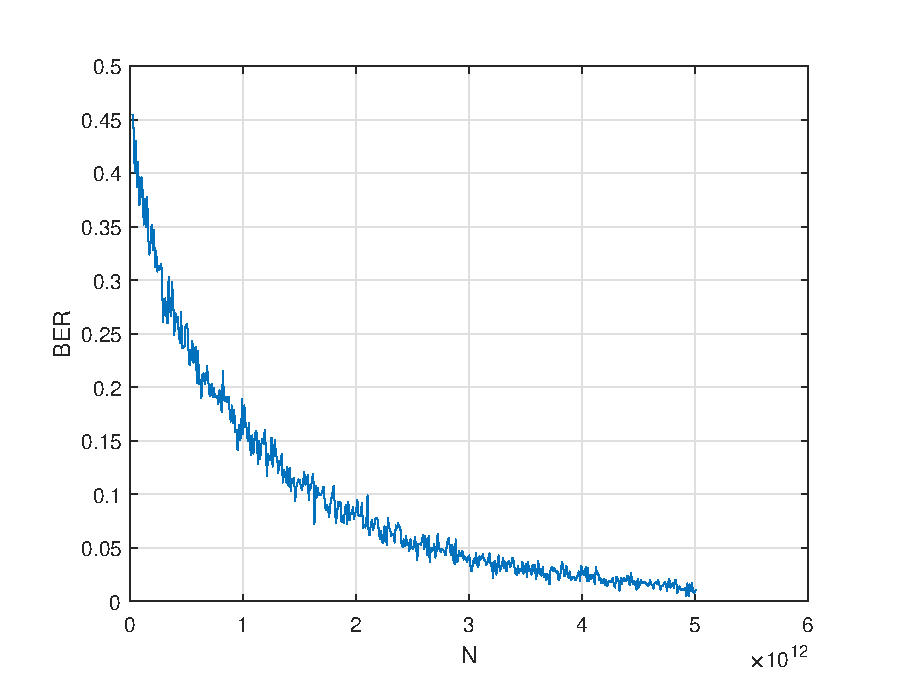
\includegraphics[height=30mm,width=40mm]{1e-6.eps}\\
$h=10^{-5}$ & $h=10^{-6}$\\
\centering
\caption{BER vs. $N$ with different $h$}
\end{tabular}

\section{Result}
BER decreases while $N$ grows. When the magnitude of $N$ reaches $10^{6}$, BER is over $15\%$. As shown in Fig.\ref{fig}, BER is inversely proportional to $N$. If we want to obtain lower BER, we can only sacrifice transmission efficiency. 

Due to the fact that BER is inversely proportional to N, it is hard to decrease when the BER is below $10\%$. If we want to get an accurate signal, $N$ should be greater than $1.6\times 10^{6}$ (BER is lower than $10\%$). However, if we need the BER below $1\%$, time consumption will increase geometrically.

When $h$ is different, we realize that $N$ is squared growing. If $h=10^{-6}$, $N$ should be more than $10^{12}$. It means that one bit information should be sent for $10^{12}$ times. Considering the communication frequency between the moon and the earth is about $40$GHz\cite{b6}, one bit information should be sent for $250$sec. The bandwidth is only $0.004$bps when $h=10^{-6}$. Here is the bandwidth when $h$ is different.
\begin{figure}[hbtp]
\centering
\vspace{-3mm}
\begin{tabular}{c|cccc}\hline\hline
$h$            & $10^{-3}$ & $10^{-4}$ & $10^{-5}$ & $10^{-6}$\\\hline
Bandwidth & 4Kbps & 40bps & 0.4bps & 0.004bps \\\hline\hline
\end{tabular}
\vspace{-3mm}
\end{figure}

From the table we know that if we have to use Multiple Signal Sending Algorithm, the $h$ should be greater than $10^{-3}$ in order to ensure the bandwidth of the communication.

\section{Conclusion}
In this paper, multiple signal sending algorithm is proposed and simulation is discussed. The multiple signal sending algorithm can acquire weak signal accurately in the problem of the earth and the moon communication. From the simulation of the algorithm, we get that the value of $N$ should be between $1.6\times 10^{6}$ to $6\times 10^{6}$ when $h=10^{-3}$, so that it can achieve both efficiency and accuracy.

The algorithm studied in this paper will be particularly useful when the signal between the earth and the moon is very weak and where white gaussian noise is the predominant noise source.

\bibliographystyle{IEEEtran}
\begin{thebibliography}{00}
\bibitem{b1} MA Li-xin, “Weak signal detection based on duffing oscillator,” International Conference on Information Management, Innovation Management and Industrial Engineering, pp. 430-433, 2008.
\bibitem{b2} Shuo Shi, Wanyi Yin, Mingchuan Yang, and Mingjie He, “A highresolution weak signal detection method based on stochastic resonance and superhet technology,” 7th International ICST conference on communications and networking, China, pp. 329-333, 2012.
\bibitem{b3} Pan Xi, "ALE-FFT algorithms for weak signal acquisition," 2010 International Symposium on Intelligent Signal Processing and Communication Systems, Chengdu, 2010, pp. 1-4, doi: 10.1109/ISPACS.2010.5704773.
\bibitem{b4} J. Sun, P. Ma, N. Zheng and J. Shi, "Study on the Signal Detection Algorithm of Weak Laser Radar Target Based on Wavelet Transform," 2010 Third International Symposium on Information Processing, Qingdao, 2010, pp. 225-227, doi: 10.1109/ISIP.2010.146.
\bibitem{b5} Montgomery, Douglas C.; Runger, George C. (2014). “Applied Statistics and Probability for Engineers (6th ed.)”. Wiley. p. 241. ISBN 9781118539712.
\bibitem{b6} NASA, "NASA's Lunar Communications and Navigation Architecture," Technology Exchange Conference, 2007.
\end{document}



